%Replace Strings:
%PROJECT.TITLE
%TODO.CHANGE
%PROJECT.ABSTRACT.KEYWORDS

\documentclass[12pt, a4paper, oneside]{article}

\usepackage[utf8]{inputenc}
\usepackage[bindingoffset=1.57cm, left=2.54cm, right=2.54cm, top=2.54cm, bottom=2.54cm]{geometry}
\usepackage{mathptmx}
\usepackage{fancyhdr}
\usepackage{lipsum}
\usepackage{secdot}
\usepackage{lastpage}
\usepackage{cite}

\tolerance=1
\emergencystretch=\maxdimen
\hyphenpenalty=10000
\hbadness=10000



\usepackage{graphicx}
	\graphicspath{ {images/} }

\usepackage{tocloft}
\usepackage[table,xcdraw]{xcolor}

\usepackage{floatrow}
\floatsetup[table]{capposition=bottom}

\linespread{1.2}
\pagestyle{fancy}
\fancyhf{} % sets both header and footer to nothing
\renewcommand{\headrulewidth}{0pt}
\rhead{ \textit{EcoCycleMart:Ecommerce for Recycled Products}}
\cfoot{\thepage}

\setlength{\parindent}{0pt}
\setlength{\parskip}{12pt}

%\frontmatter

\begin{document}

\pagenumbering{roman}
\addcontentsline{toc}{section}{Abstract}
\large
\begin{center}
	\textbf{ABSTRACT}
\end{center}

\normalsize
Environment is the major source of industrial raw materials. The heavy need of raw materials has been burden for the environment. In the other hand, waste management has been another big issue. This has made us environmentally conscious than ever. We can reduce dependency on environment for raw materials by recycling. For example, Recycling paper reduces the demand for trees to be cut down. Recycling is less energy consuming than manufacturing from scratch. Manufacturing leads to heavy green house gas emissions while the recycling significantly reduces it. Recycling is cost efficient.

EcoCycleMart is the e-commerce platform for the recycled eco-friendly goods where the sellers can list their goods and the buyers can purchase them. The project aims to provide help to the small and medium scale recycling based businesses to find the consumer for their goods. It also ensures consumers, the best quality goods in affordable price. In the long run, the project sets its objective to aware and encourage everyone to use the recycled products for noble cause of environmental protection and sustainability of resources. In summary, this project promotes low capital business, ensures fulfillment of needs for quality products without exploiting environment for resources and minimize the waste management issues.

The major deliverable proposed in the project is a web based application with
user-friendly User Interface and AI based recommendation system .

\textbf{Keywords}: Environment, Waste, Recycle, E-commerce, EcoCycleMart \\

\break

\large
\addcontentsline{toc}{section}{Table of Contents}
\begin{center}
	\textbf{TABLE OF CONTENTS}
\end{center}


\normalsize
\setlength{\cftbeforetoctitleskip}{0pt}
\renewcommand{\contentsname}{}
\tableofcontents

\break

%\mainmatter
\cfoot{\textbf{\thepage} /  \pageref{LastPage}}

\pagenumbering{arabic}
\section{Introduction} 
EcoCycleMart is a web based application that provides platform for selling and buying recycled goods.With a view of encouraging the use of recycled goods, the application  aims to fulfill needs for quality goods without exploiting the environment for resources and minimize the waste management issues.In the long term, 
 it targets to conserve environment and maintain ecological balance.This document looks forward to providing essential information about the needs, scope, objectives and proposed methodology of the application.

E-commerce has a great potential to contribute to the economy and prosperity of nation, but having observation at the statistics, the ratio of contribution of e-commerce is not satisfactory. The recycle based e-commerce market is almost negligible in Nepal. According to Nepal Rastra Bank, the total contribution of the e-commerce to the total GDP of Nepal was almost \$600 million comprising just above than 1\% in 2022/2023.

The government of Nepal has taken efforts to promote recycle based e-commerce. Taking this in consideration the authors have proposed to build the e-commerce web application specially tailored for the low capital recycle based business and consumers looking for goods at affordable price.

The impact on the environment is severe due to the industries . The issues like
climate change, global warming, greenhouse effects etc has made our planet the ill place to live. In the other hand the waste have been everywhere not managed and left alone. So, why not make use of this thing and contribute towards making earth good place to live.

\subsection{Problem Statement}
In today's consumer-driven society, the massive production and disposal of goods have led to a significant burden on our planet's resources and ecosystems. The linear 'take-make-dispose' model of production and consumption leads to environmental degradation, invites climate change, and accelerates the depletion of finite resources. Despite growing awareness of these issues, there remains a lack of accessible and convenient options for individuals to adopt more sustainable consumption habits. Furthermore, while recycling is recognized as a crucial component of sustainable waste management, there exists a disconnect between the availability of recycled products and consumer demand.

\subsection{Project Objectives}
The proposed project has put forward the following objectives:

\begin{itemize}
	\item To make the sustainable alternative for e-commerce more accessible and convenient.
	\item To promote the local small and medium scale recycle based e-commerce .
	\item To aware consumers about the environmental impact of their purchasing choices and the benefits of opting for recycled products.
\end{itemize}

\subsection{Significance of the Study}
The project proposed is significant owing to the fact that we are living in digital world, and the proposed project will certainly be fruitful in achieving the objectives set by the Government of Nepal regarding Ecological Balance, Waste management and promoting ecommerce. Since the proposed idea is one of the first of its kind, it is expected that the project will reach to a significant majority of sellers and buyers.

\subsection{Scope and Limitations}
In the beginning phase, the basic e-commerce concept will be implemented and other features are proposed to be added later gradually if possible. Such possible extensions could be addition of google authentication, chat bots, AI based recommendation for products, payment integration, rating and reviews etc. The sellers will be able to make their accounts including profiling and list their products in the platform. The buyers can wishlist, add to cart and purchase the products. The users can signin/signup using their google account. They can also rate and review the products. The buyers and sellers both will have separate dashboards. The application will be able to process payments using the feasible payment providers/services in Nepal. 

The following are the limitations of the project that are realized:
\begin{itemize}
 	\item The application will be web based but native applications such as mobile and desktop application will not be built.
	\item The application will not be able to ensure the quality and detect if the product being listed is recycled or not .
	\item The application will have the order tracking but logistics aspect will not 
be incorporated.	
 \end{itemize}

\break
\section{Literature Review}
This section consists description of the literature study performed during the development of this proposal.

\subsection{Paper Recycling by Jamarko}
Jamarko was established in 2001 as a small cottage industry with the view of contributing towards environmental conservation and to provide employment to the underprivileged, especially women.While Jamarko’s short-term objective is to minimize the amount of waste paper,the long-term goal is to help conserve natural resources and habitats, and promote local handmade products.
At Jamarko, they collect paper waste from various sources, and recycle them to produce recycled paper products.Its official website (https://jamarko.com.np/) is aimed at providing a platform for buying and selling of recycled products
digitally.

\subsection{GoodTrade Magazine's view on recycle based E-commerce}
Seeking out ethical online marketplaces to purchase our recycled products helps support
businesses that prioritise ethical practices, sustainability, and social responsibility. Giant online
retailers like Amazon and Wish have faced criticism for their environmental impact, labour
practices, and monopolistic tendencies, raising concerns about the ethics of supporting such
platforms. Actively choosing to shop at ethical marketplaces helps our capital reach
marketplaces that value and respect sustainable business practices and fair labour practices. 

\subsection{Existing Similar Appilcations}
While EcoCycleMart carves its niche in the sustainability landscape, let's delve deeper into existing solutions with distinct platforms:

Material Marketplaces: \\
Platforms like Material Exchange ( https://material-exchange.com/ ) and Loop ( https://exploreloop.com/shop/ ) focus on connecting businesses with recycled materials for industrial use. They provide a B2B marketplace for manufacturers seeking to incorporate recycled content into their products.\\
Strengths: High volume transactions, facilitates large-scale recycling integration.\\
Weaknesses: Not targeted at individual consumers.

Curated Recycling Platforms:\\
 Project Regeneration ( https://regeneration.org/ ) offers a curated online marketplace for high-end, designer furniture crafted from recycled materials. They partner with skilled artisans who transform salvaged materials into unique pieces.\\
Strengths: Promotes high-quality, one-of-a-kind recycled products, caters to a specific design-conscious audience.\\
Weaknesses: Limited product variety, potentially higher price points\\

Hyperlocal Recycling Initiatives:\\
 Apps like Bunz ( https://www.bunz.com/ ) or Freecycle ( https://www.freecycle.org/ ) facilitate localized exchange of unwanted items, including some recycled goods. They foster a hyperlocal community feel and promote a sharing economy.\\
Strengths: Encourages reuse and community building, reduces transportation needs.\\
Weaknesses: Limited product selection, can be challenging to find specific recycled items due to the non-curated nature. 
These existing solutions, with their distinct platforms, highlight various approaches to promoting recycling. However, they often cater to specific niches or lack the comprehensive focus on individual consumer-to-consumer buying and selling of a wide range of recycled goods that EcoCycleMart aims to achieve.

%\subsection{Challenges}
%One of the major challenges realized is the validation of the collection of treasures by the users. If only QR code is used for validating that a tourist has in fact reached a destination, there is a high chance that the QR codes get shared among people and people will remotely validate themselves having gone to a place and collected a treasure just by scanning the photo of the QR from a remote location. A countermeasure that can be used is to add actual location data from the user's phone's GPS sensor as an additional parameter for validation. A treasure is only considered to be collected if a user scans the QR from within a specific distance from the actual treasure location.
%
%GPS spoofing is one of the major challenges for any system that has used GPS for the validation. GPS spoofing is the process of modifying a GPS receiver unit so that it broadcasts incorrect GPS signal. Some countermeasures to tackle GPS spoofing are monitoring absolute as well as relative GPS signal strength; checking time intervals and performing comparision; and performing sanity checks \cite{gpsspoofmeasures}.

\break
\section{Proposed Methodology}
This section describes the methodology that is proposed to be followed during the development of the project.

\subsection{Proposed Software Development Life Cycle}
The project will be developed as per iterative and incremental model of software development life cycle as depicted in Figure \ref{fig:sdlc}. The reason for choosing this model is its cyclic approach and adaptive flexibility, as well as very high chances of the changes of requirements in the process of development. 

\begin{figure}[h]
	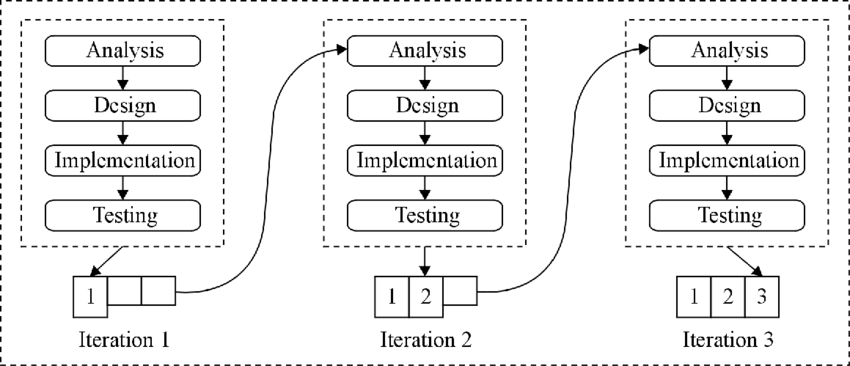
\includegraphics[width=\linewidth]{sdlc}
	\centering
	\caption{Proposed software development life cycle(Iterative and Incremental Approach)}
	\label{fig:sdlc}
\end{figure}

The life cycle begins with the first iteration, when the team collects and evaluates the requirements that will be expected from the application. The design and\\ implementation phase will be to design and build both backend and client side applications. By the end of this iteration, a Minimal Viable Product (MVP) will already have been constructed. In the testing and debugging phases, the quality control methods will be applied to both frontend and backend. If any changes in requirement are needed, then it can send feedback to the analysis phase that will mark the beginning of the new iteration. The project is expected to be completed in 3 iterations.
 

\subsection{Technical Architecture}
The application will be built upon the client-server web architecture, as illustrated in Figure \ref{fig:arch}.

\begin{figure}[h]
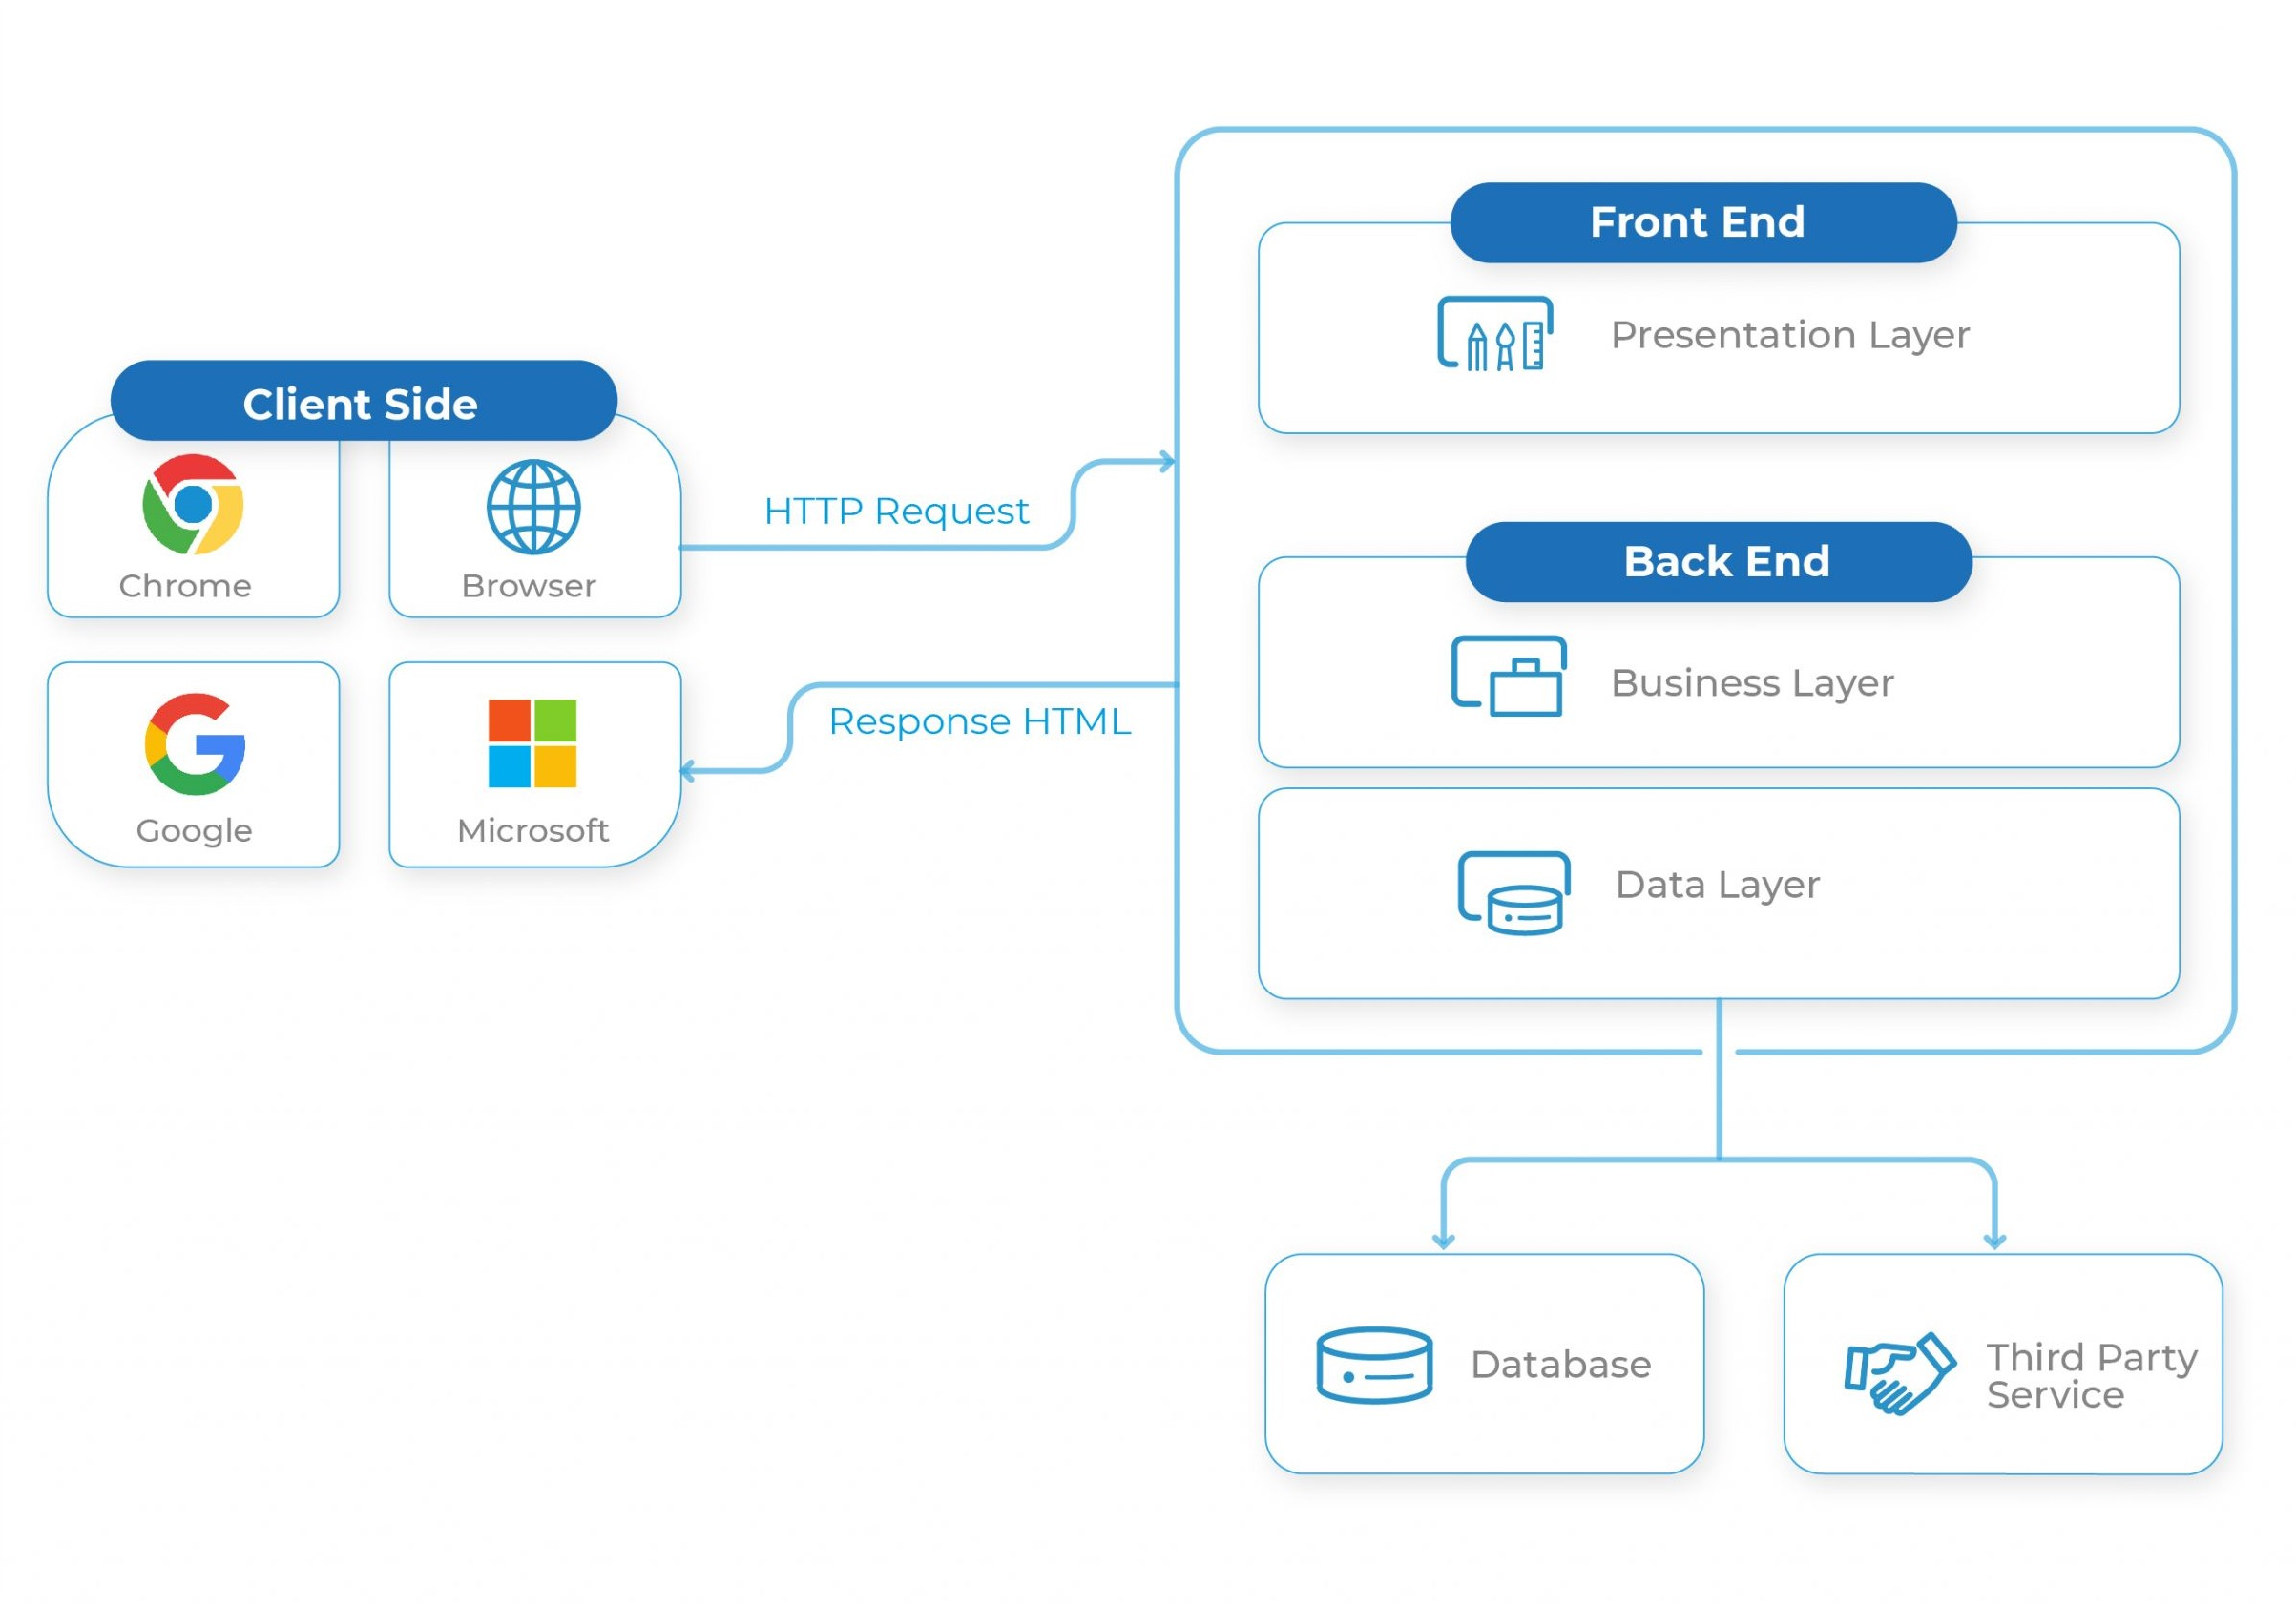
\includegraphics[width=\linewidth]{architecture}
\centering
\caption{Proposed architecture of the application}
\label{fig:arch}
\end{figure}

At the heart of the architecture lies the RESTful web service which communicates directly with the central database where all the data is stored. The client application  do not access the database directly, but via the API service. The clients send HTTP requests like GET, POST, PUT and DELETE while the API service processes those requests and return the data in JSON format. 


\subsection{Proposed Technologies}
Table \ref{table:tech} consists of the major technologies that are proposed to be used during development and deployment of the application.

\renewcommand{\arraystretch}{1.5}
\begin{table}[]
\begin{tabular}{|l|l|}
\hline
\rowcolor[HTML]{C0C0C0} 
\textbf{Subject}    & \textbf{Proposed Technology}   \\ \hline
Database            & MongoDB                       \\ \hline
REST API Service    & Express REST Framework         \\ \hline
Frontend            & ReactJs                        \\ \hline
Backend             & NodeJs, ExpressJs             \\ \hline
Admin Web Interface & ReactJs              \\ \hline
%Deployment Platform & Amazon Web Services (AWS)      \\ \hline
Documentation & LaTeX \\ \hline
\end{tabular}
\caption{Technologies proposed to be used}
\label{table:tech}
\end{table}


\pagebreak
. \pagebreak
\section{Proposed Deliverables}
The following will be the major deliverables that will be produced at the end of this project.

\subsection{RESTful API service}
There will be a running instance of RESTful API service developed and deployed at the end of the project. This API will be responsible for communicating between the client applications and the central database server.

\subsection{Frontend and Admin Dashboard}
The application will be developed integrating all the features proposed earlier. The sellers will be able to use the application to list their products which will be visible to the buyers. An interactive chat box will be integrated with the application that will allow the users to make queries. The application will also be integrated with google authentication, payment processing, AI based recommendation system. The application will be featured with order tracking abilities. 



\break
\section{Project Task and Time Schedule}
The working time period for the project is less than three months. The project will be completed by the end of the spring semester as per the requirements of the university. The major task division among the team members is mentioned in Table \ref{table:taskdiv}.

\begin{table}[h!]
\begin{tabular}{|l|l|}
\hline
\rowcolor[HTML]{C0C0C0} 

\textbf{Team Member} & \textbf{Assigned Tasks}                                                                                                                     \\ \hline
Rishikesh Sharma       & \begin{tabular}[c]{@{}l@{}} Project Management \\ AI Implementation \end{tabular} \\ \hline
Hansika Jha   & \begin{tabular}[c]{@{}l@{}}Frontend Design \\ Project Documentation\end{tabular}                                           \\ \hline
Sandip Shah   & \begin{tabular}[c]{@{}l@{}}Frontend Development\\ Project Documentation\end{tabular}                                           \\ \hline
Kishore Budhathoki  & \begin{tabular}[c]{@{}l@{}}Backend Development\\ Data Management\\
 \end{tabular}                                           \\ \hline
\end{tabular}
\caption{Division of tasks among project team members}
\label{table:taskdiv}

\end{table}


\break
The time schedule proposed for the development of the project is illustrated in table \ref{table:schedule}.

\begin{table}[h!]
\begin{tabular}{|l|c|c|c|c|}
\hline
\rowcolor[HTML]{C0C0C0} 
\textbf{Task} & \textbf{1st Iteration}                                                                                                                    & \textbf{2nd  Iteration }  & \textbf{3rd Iteration }  & \begin{tabular}[c]{@{}l@{}} \textbf{Duaration} \\ \textbf{(in days)} \end{tabular} \\ 
\hline
\begin{tabular}[c]{@{}l@{}} Requirement Analysis \\ and Specification \end{tabular}   & 3 & 2 & 3 & 8 \\
\hline
\begin{tabular}[c]{@{}l@{}} Undertake Analysis \\ of System \end{tabular}   & 2 & 2 & 3 & 7  \\
\hline
\begin{tabular}[c]{@{}l@{}} Design
System \end{tabular}   & 4 & 3 & 3 & 10 \\
\hline
\begin{tabular}[c]{@{}l@{}} Produce Requirement \\ Specification \end{tabular}   & 4 & 3 & 4 & 11 \\
\hline
\begin{tabular}[c]{@{}l@{}} Testing and Debugging \end{tabular}   & 3 & 4 & 2 & 9 \\
\hline
\begin{tabular}[c]{@{}l@{}} Overall System Test \end{tabular}   & 3 & 2 & 2 & 7 \\
\hline
\begin{tabular}[c]{@{}l@{}} Develop Documentation \end{tabular}   & 3 & 2 & 3 & 8 \\
\hline
\begin{tabular}[c]{@{}l@{}} Total days \end{tabular}   & 22 & 18 & 20 & 60 \\
\hline
\end{tabular}
\caption{Project Task and Schedule}
\label{table:schedule}
\end{table}

%\begin{figure}[h!]
%	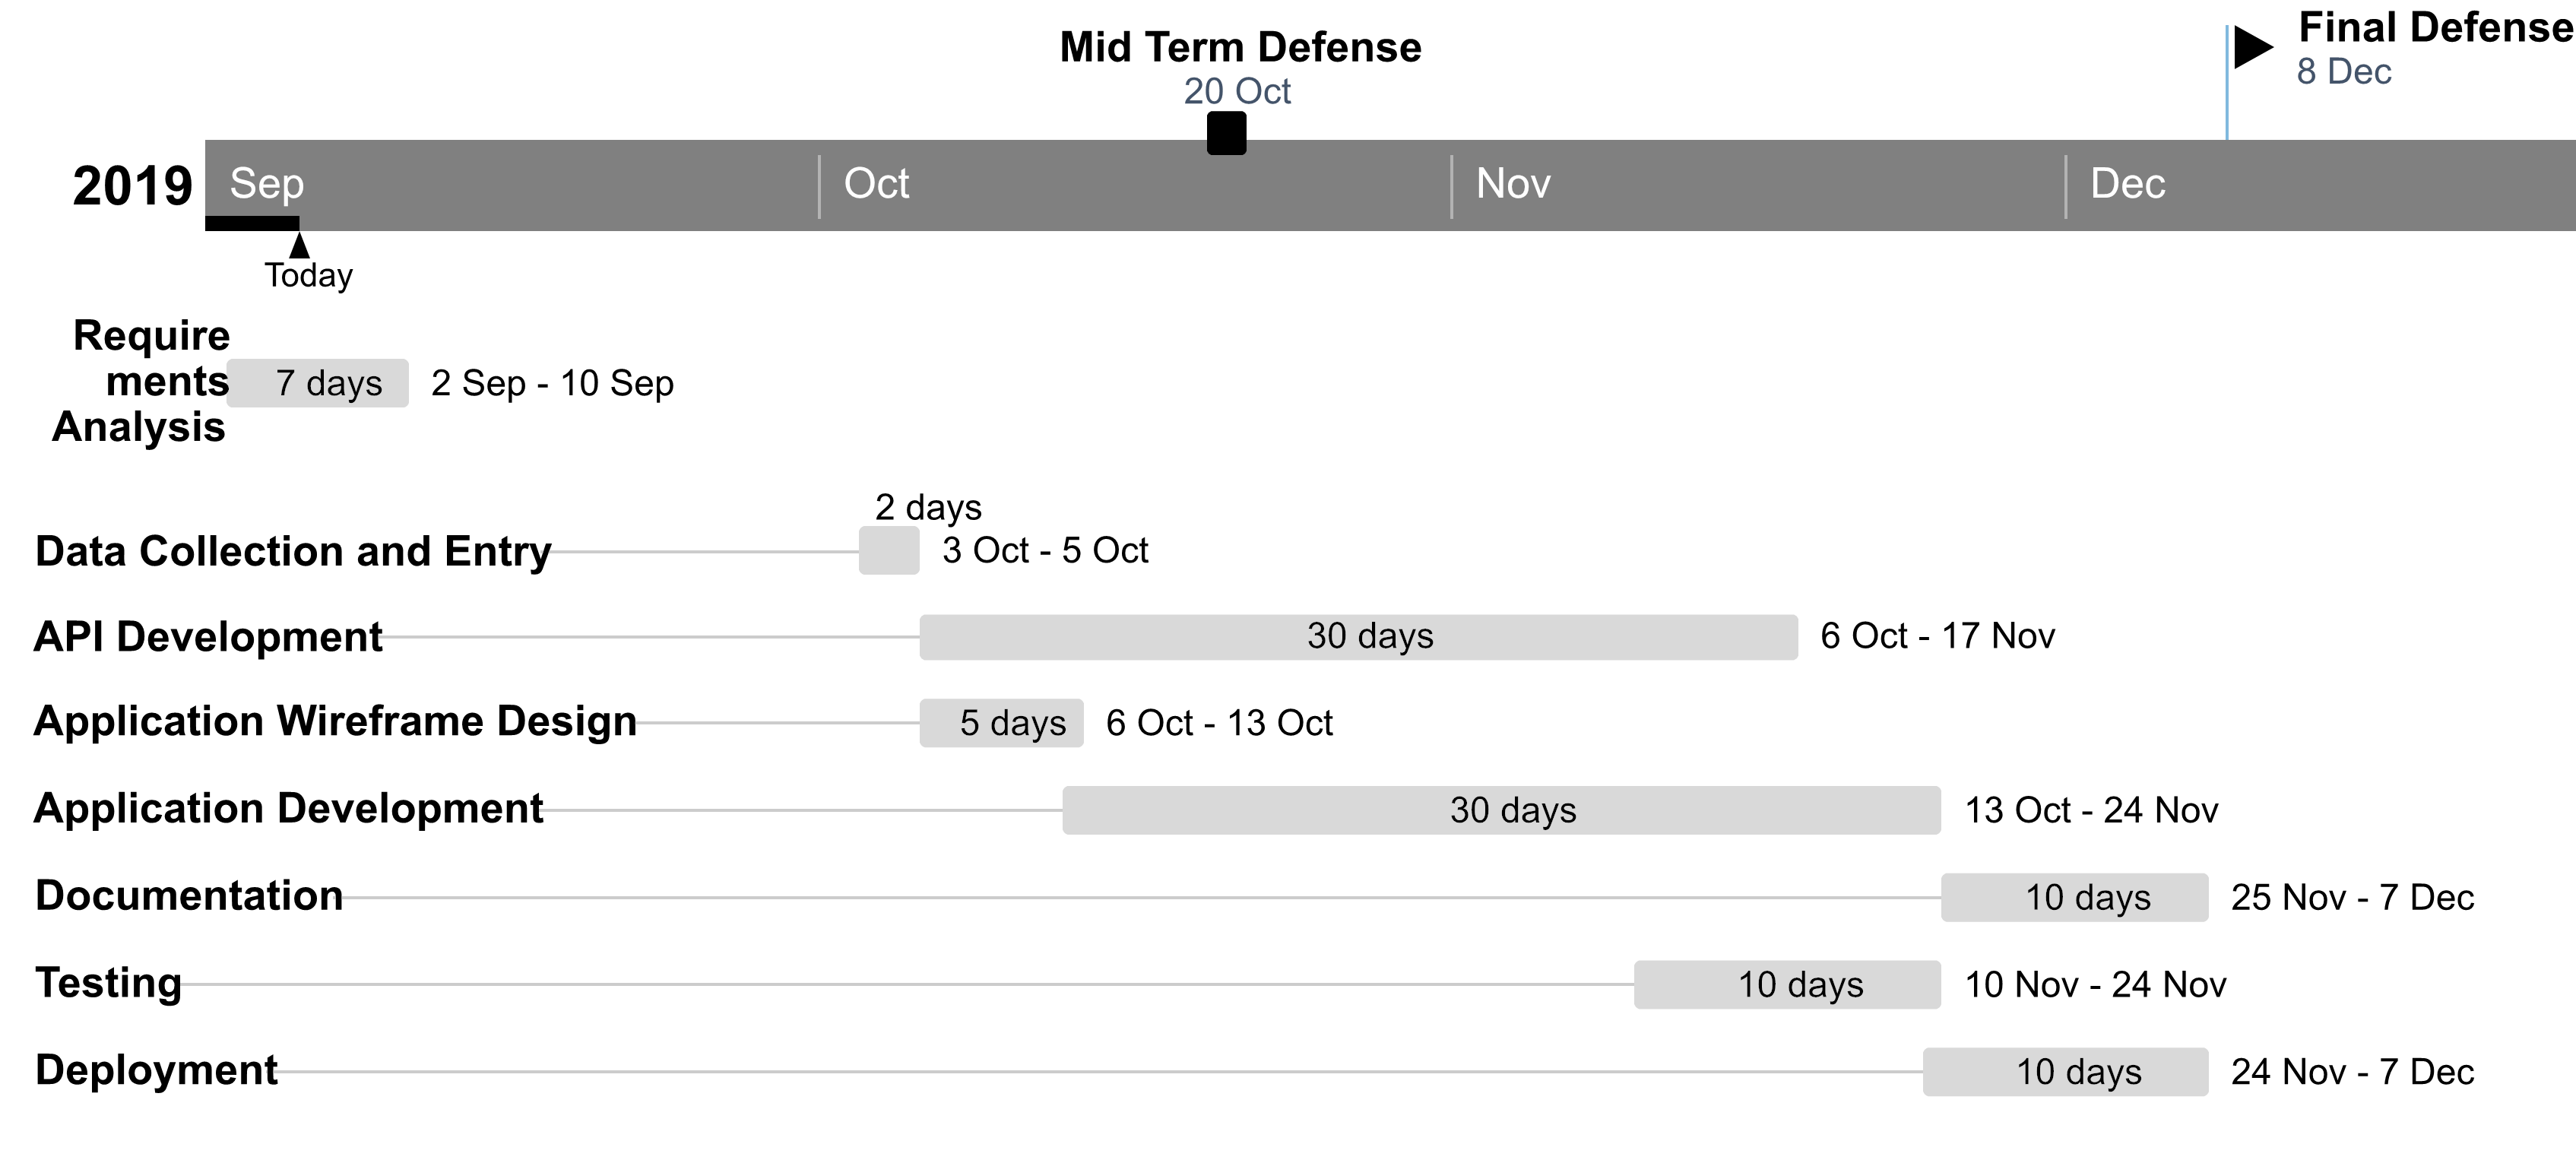
\includegraphics[width=\linewidth]{schedule}
%	\centering
%	\caption{Proposed project schedule}
%	\label{fig:schedule}
%\end{figure}


%\pagebreak
. \pagebreak
%\break
\section{References}
\bibliography{references}
\bibliographystyle{ieeetran}
@misc{GeoTrust,
title={Creating an E-Commerce web site},
place={california},
url={https://www.geotrust.com/resources/guides/creating-ecommerce-website.pdf},
year={2010}
},

@misc{journal,
title={The Role of E-Commerce in Sustainable Supply Chain Management},
publisher={Xiutian Shi et al},
year={2019},
}

@misc{similarapps,
title={Jamarko},
url={https://jamarko.com.np/},
journal={MakeUseOf},
description={
Online website for selling recycled paper material goods in Nepal.
},
}

@article{cirlulareconomy,
  title={Circular Economy Principles},
  author={Warner, Jon S and Johnston, Roger G},
  institution={Ellen MacArthur Foundation},
  description={Provides Insights and resources on circular economy principles},

}

@article{reactjs,
title={A Comprehensive Guide to React.js},
url={https://flaviocopes.com/react/},
author={Flavio Copes},
year={2021}
}


@misc{nodejstutorial,
title={Node.js Tutorial for Beginners  Learn Node in 1 Hour},
url={https://www.youtube.com/watch?v=TlB\_eWDSMt4},
year={2018}
}

\end{document}

\break
\section{Proposed Performance Analysis Methodology}
%The performance analysis of the deliverables will be performed according to the popular Top Down Methodology. The main idea in this method is to analyse and address the higher order performance issues at first, then follow the lead upto the lower levels of details if needed \cite{tdmethod}. This methodology is proposed to be followed because it largely reduces the time and cost of assessing the performance since not every modules and sections of the project need to be analyzed at a deeper level.
%
%The final evaluation of the project will be performed by the project evaluation team designated by the college administration.
